\documentclass[no-math,zihao = -4]{ctexart} %由于前置宏包的需求,强烈建议使用ctexart且加上"no-math,zihao = -4"的设置。
\usepackage{spaexptemp} % 使用 StarHub-SPA 实验模版宏包


%====待填信息,这部分内容请使用时据实际修改第二个大括号的内容====%
\newcommand{\exptitle}{CC1+A 热辐射的测量设计性实验} %建议输入完整的实验名称
\newcommand{\stid}{1XXXXXXX} %输入自己的学号
\newcommand{\major}{XX学} %填入专业信息:如"物理学"
\newcommand{\grade}{20XX级} %年级
\newcommand{\name}{张三} %你的名字


%====正文处模版(非固定样式)====%
\begin{document}
\kaitou % 排版开头打分表等表格信息。请填写好待填信息。

\section{背景介绍}
    一入\TeX 深似海,用起来十分的开心,但是每次写\TeX 都是从
    \verb|\documentclass{ctexart}|
    开始,而且丰富多彩的宏包总会产生吃岁月湖麻辣烫时一样的选择恐惧症。而且市面上暂时(我)未找到十分心满意足轻量的实验报告模板。
    于是就有了这么一个妖孽所在。这个Simple仅仅只介绍一些很基础、日常的用法,更加高级的排版还是需要各位阅读更系统更专业的\TeX 教程书籍。

    \subsection{实验目的}
        \begin{enumerate}
            \item 第一个目的
            \item 第二个阴谋
        \end{enumerate}

    \subsection{实验仪器}
        \begin{center}
            \begin{tabular}[c]{cccc}
                \toprule
                    编号   &仪器用具名称 &  数量   &主要参数(型号,规格等)\\ 
                \midrule
                    1    & 脑子   & 1 & AE86  \\ 
                    2    & 腿  & 2 & 11 \\ 
                \bottomrule
            \end{tabular}
            \captionof{table}{实验的用具}
            \label{tab:实验用具}
        \end{center}

    \subsection{实验注意事项}
        \begin{enumerate}
            \item 注意人生安全
            \item 记得吃饭
            \item 记得睡觉
            \item 记得喝水
            \item 记得呼吸
        \end{enumerate}
\section{原理概述}
    \subsection{人被杀为什么会死}
        因为人被杀了之后,\autoref{tab:实验用具} 的仪器无法使用,就无法进行生理活动,于是乎就不能上实验课,就会于心有愧致死。

    \subsection{预习思考题}
        \begin{enumerate}
            \item 你为什么这么骚?
            \begin{ans}
                我也不是很清楚,大概就是天赋把。
            \end{ans}

            \item 为什么你自己骚还要告诉别人?
            \begin{ans}
                我也不知道,大概就是欲望把。
            \end{ans}
        \end{enumerate}
\section{实验步骤}
    \subsection{多个小实验的其中之一}
        \begin{enumerate}
            \item 进入实验室。
            \item 缓缓坐下来,手提着书包,但是缓缓放下来在地面上。
            \item 迅速从书包中拿出实验报告,然后眼睛看着实验报告右前方约10度角距的位置。
            \item 展现出若有所思的眼神约2分钟。
            \item 拿着报告迟疑的走向老师,询问老师一些问题
                \begin{enumerate}
                    \item 老师这个电源为什么没反应?
                    \item 老师这个量这样测不会引入很多误差吗?
                    \item 老师这个结论为什么的这样,应该还会有另外一种情况吧?
                    \item 老师这个数据处理方式应该不是很普遍吧?
                \end{enumerate}
            \item 掩盖自己完全没有预习的慌张的同时,把实验搞清楚要怎么做。
            \item 完成记录数据\autoref{tab:实验1表格}
            \item 下课前40分钟,把实验数据给老师看,有问题就改,反复3次,就可以提早吃饭了。
        \end{enumerate}
    \subsection{多个小实验的其中之二}
        \begin{enumerate}
            \item 实验下课后,走到隔壁小伙伴的身旁
            \item 问他
                \begin{itemize}
                    \item 我算的数据误差好大,你怎么算的?
                    \item 这个思考题你在哪里找的答案?
                    \item 你这个图怎么画的?
                \end{itemize}
            \item 根据回答完成实验报告,提交。
        \end{enumerate}

\section{实验数据记录及处理}
    \subsection{多个小实验的其中之一}
        这里可能需要记录一些额外的东西\autoref{tab:实验1表格}
        
        \begin{table}[h]
            \ct
            \at{1.3}
            \caption{人美字好看的数据记录表格}
            \label{tab:实验1表格}

            \begin{tabularx}{0.85 \textwidth}{|*{6}{>{\ct \ar}X|}}
                \toprule
                实验人员:& \multicolumn{2}{c|}{}&相机ISO&\multicolumn{2}{c|}{} \\ \hline
                测量值 &1 & 2 & 3 & 4 & 5\\
                \midrule
                身高$(\bm{N})$ &&&&&\\ \hline
                体重$(V)$ &&&&&\\
                \bottomrule
            \end{tabularx}
        \end{table}

        \begin{gather}
            a = c \\
            d = b
        \end{gather}

        \begin{align}
            a + b &= a + b \\
            &= c + d    \label{eq:cal}
        \end{align}
    \subsection{多个小实验的其中之二}
        不重复演示了

    \clearpage
    \newpage

\section{分析与讨论}
    \subsection{我想讨论的第一个事情}
        我用相机进行了神秘操作测量了自己的身高与体重,如\autoref{tab:实验1数据}
        \begin{table}[h]
            \ct
            \caption{身高体重测量数据}
            \label{tab:实验1数据}

            \begin{tabularx}{0.85\textwidth}{*{6}{>{\ct \ar}X}}
                \toprule
                测量值 &1 & 2 & 3 & 4 & 5\\
                \midrule
                身高$(\bm{cm})$ & 180 & 182 & 181 & 183 & 180\\ \hline
                体重$(kg)$ & 68 & 68 & 67 & 68 & 68 \\
                \bottomrule
            \end{tabularx}
        \end{table}

        实验数据所测非常精准,根据\autoref{eq:cal} 用得到的数据作图,可以得到\autoref{fig:实验1数据图}
        
        \begin{figure}[h]
            \ct
            \caption{数据绘图}
            \label{fig:实验1数据图}
            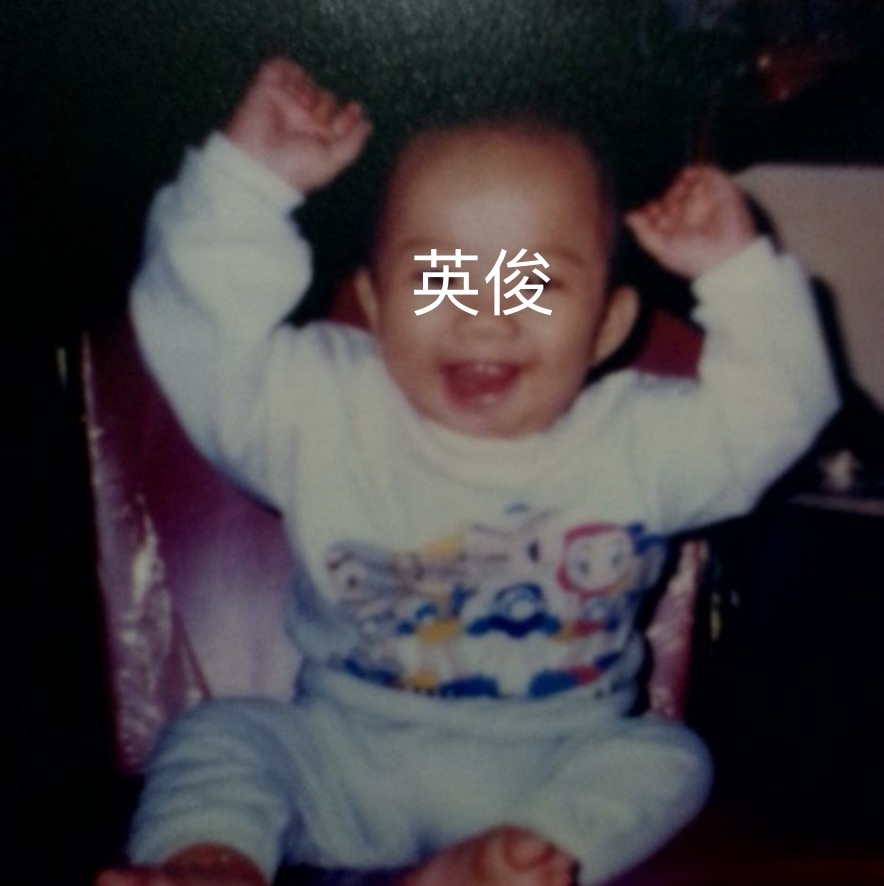
\includegraphics[width = 0.5\textwidth]{./img/data1.png}
        \end{figure}

        由图中可以明显看出一个趋势
        \begin{conc}
            图中人物十分英俊。
        \end{conc}

        还有一个不怎么显然,但是也可以证明的结论。
        \begin{conc}
            图中人物十分年轻
        \end{conc}

        \newpage
        \subsection{实验后思考题}
            \begin{enumerate}
                \item 为什么你觉得你测量出了身高与体重就能得到相应的结论?
                    \begin{ans}
                        我不要你觉得,我要我觉得。
                    \end{ans}
            \end{enumerate}


\end{document}